\begin{center}
\begin{tikzpicture}
    \node[anchor=south west,inner sep=0] (image)  at (0,0) {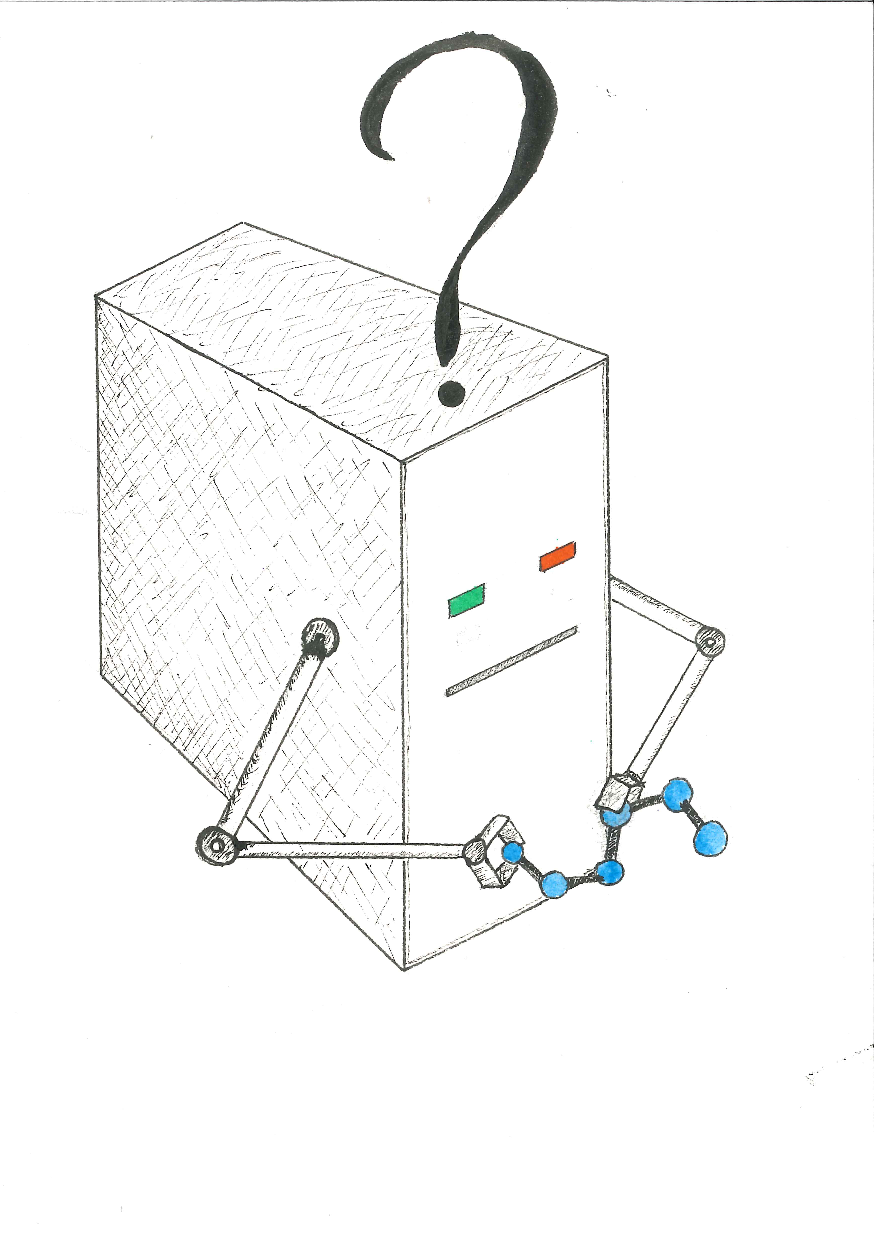
\includegraphics[trim={2mm, 2mm, 2mm, 2mm}, width=0.995\pagewidth]{scans/pg_0006.pdf}};

    \begin{scope}[x={(image.south east)},y={(image.north west)}]
        \if\helplines1
        	\draw[help lines,xstep=.1,ystep=.1] (0,0) grid (1,1);
        \fi
        \node[align=center, anchor=north](0) at (0.5, 0.15) {\english{\Large But, how does a computer know how to fold proteins?}};
        
        \node[align=center, anchor=north](0) at (0.5, 0.09) {\spanish{\Large Pero, ¿cómo sabe el ordenador cómo plegar proteínas?}};
    \end{scope}

\end{tikzpicture}
\end{center}